\documentclass{standalone}
\usepackage{tikz}
\usetikzlibrary{patterns, positioning}


\begin{document}
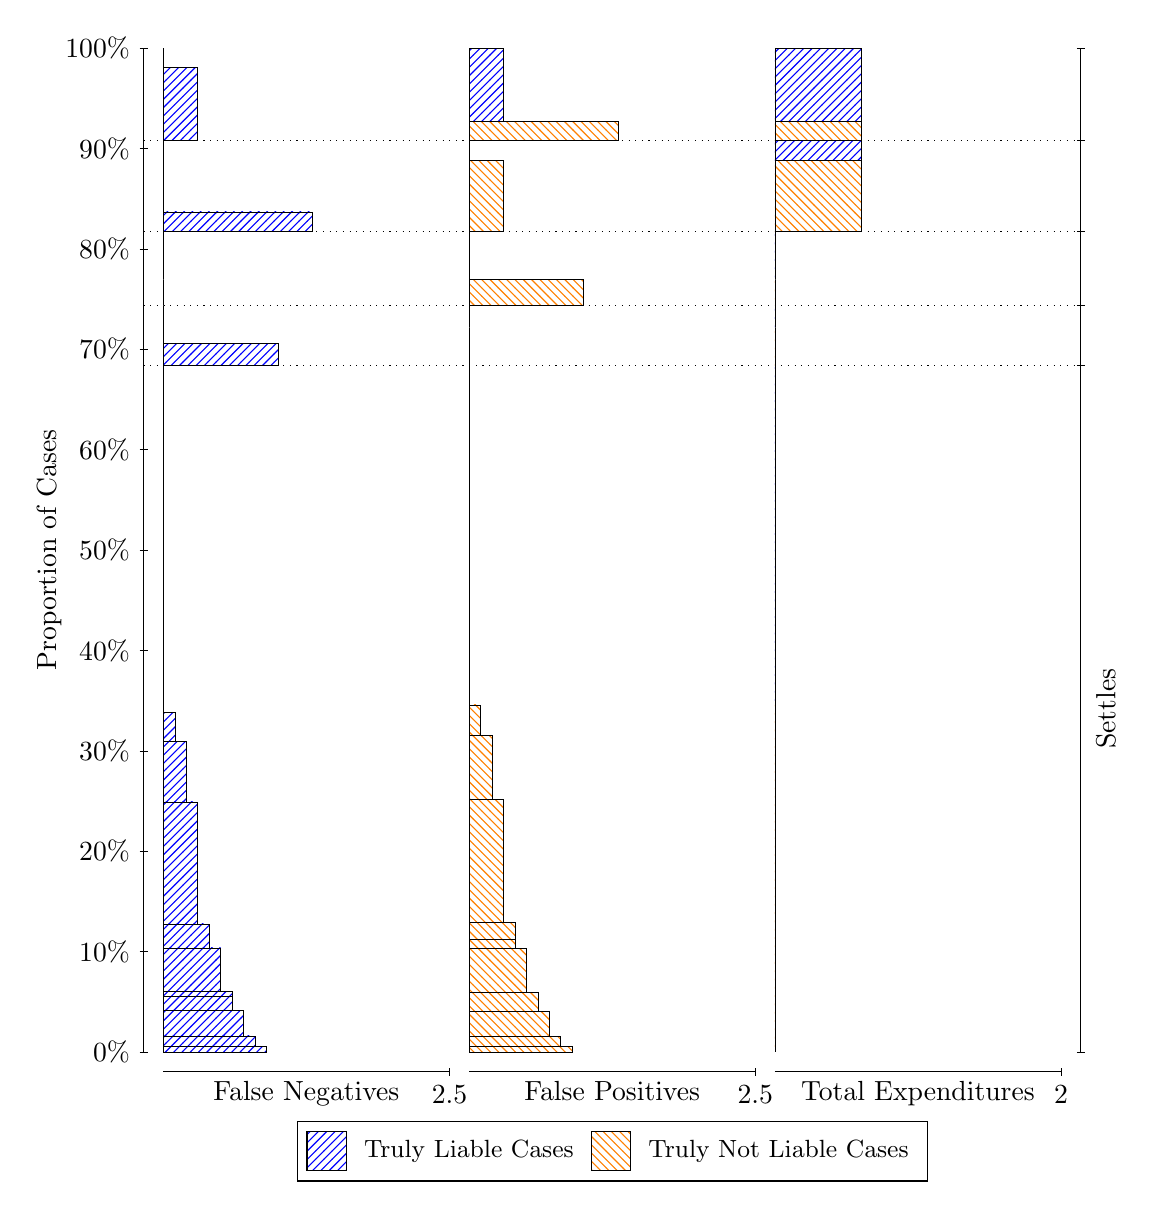
\begin{tikzpicture}
\draw[black, very thin] (1.5,1.75) -- (1.5,14.5);
\node[rotate=90, text=black, anchor=center] at (0.3, 8.125) {Proportion of Cases};
\draw[black, very thin] (1.45,1.75) -- (1.55,1.75);
\node[text=black, anchor=east] at (1.45, 1.75) {0\%};
\draw[black, very thin] (1.45,3.025) -- (1.55,3.025);
\node[text=black, anchor=east] at (1.45, 3.025) {10\%};
\draw[black, very thin] (1.45,4.3) -- (1.55,4.3);
\node[text=black, anchor=east] at (1.45, 4.3) {20\%};
\draw[black, very thin] (1.45,5.575) -- (1.55,5.575);
\node[text=black, anchor=east] at (1.45, 5.575) {30\%};
\draw[black, very thin] (1.45,6.85) -- (1.55,6.85);
\node[text=black, anchor=east] at (1.45, 6.85) {40\%};
\draw[black, very thin] (1.45,8.125) -- (1.55,8.125);
\node[text=black, anchor=east] at (1.45, 8.125) {50\%};
\draw[black, very thin] (1.45,9.4) -- (1.55,9.4);
\node[text=black, anchor=east] at (1.45, 9.4) {60\%};
\draw[black, very thin] (1.45,10.675) -- (1.55,10.675);
\node[text=black, anchor=east] at (1.45, 10.675) {70\%};
\draw[black, very thin] (1.45,11.95) -- (1.55,11.95);
\node[text=black, anchor=east] at (1.45, 11.95) {80\%};
\draw[black, very thin] (1.45,13.225) -- (1.55,13.225);
\node[text=black, anchor=east] at (1.45, 13.225) {90\%};
\draw[black, very thin] (1.45,14.5) -- (1.55,14.5);
\node[text=black, anchor=east] at (1.45, 14.5) {100\%};

\draw[black, very thin] (13.4,1.75) -- (13.4,14.5);
\draw[black, very thin] (13.35,1.75) -- (13.45,1.75);
\node[anchor=west] at (13.35, 1.75) {};
\draw[black, very thin] (13.35,10.471) -- (13.45,10.471);
\node[anchor=west] at (13.35, 10.471) {};
\draw[black, very thin] (13.35,11.23) -- (13.45,11.23);
\node[anchor=west] at (13.35, 11.23) {};
\draw[black, very thin] (13.35,12.17) -- (13.45,12.17);
\node[anchor=west] at (13.35, 12.17) {};
\draw[black, very thin] (13.35,13.324) -- (13.45,13.324);
\node[anchor=west] at (13.35, 13.324) {};
\draw[black, very thin] (13.35,14.5) -- (13.45,14.5);
\node[anchor=west] at (13.35, 14.5) {};

\draw[black, very thin, pattern color=blue, pattern=north east lines] (1.75,1.75) rectangle (3.058,1.8214);
\draw[black, very thin, pattern color=blue, pattern=north east lines] (1.75,1.8214) rectangle (2.9127,1.9543);
\draw[black, very thin, pattern color=blue, pattern=north east lines] (1.75,1.9543) rectangle (2.7673,2.2799);
\draw[black, very thin, pattern color=blue, pattern=north east lines] (1.75,2.2799) rectangle (2.622,2.4582);
\draw[black, very thin, pattern color=blue, pattern=north east lines] (1.75,2.4582) rectangle (2.622,2.5231);
\draw[black, very thin, pattern color=blue, pattern=north east lines] (1.75,2.5231) rectangle (2.4767,3.0725);
\draw[black, very thin, pattern color=blue, pattern=north east lines] (1.75,3.0725) rectangle (2.3313,3.3781);
\draw[black, very thin, pattern color=blue, pattern=north east lines] (1.75,3.3781) rectangle (2.186,4.9263);
\draw[black, very thin, pattern color=blue, pattern=north east lines] (1.75,4.9263) rectangle (2.0407,5.6974);
\draw[black, very thin, pattern color=blue, pattern=north east lines] (1.75,5.6974) rectangle (1.8953,6.0614);
\draw[black, very thin, pattern color=orange, pattern=north west lines] (1.75,6.0614) rectangle (1.75,10.471);
\draw[black, very thin, pattern color=blue, pattern=north east lines] (1.75,10.471) rectangle (3.2033,10.748);
\draw[black, very thin, pattern color=orange, pattern=north west lines] (1.75,10.748) rectangle (1.75,11.23);
\draw[black, very thin, pattern color=orange, pattern=north west lines] (1.75,11.23) rectangle (1.75,11.561);
\draw[black, very thin, pattern color=blue, pattern=north east lines] (1.75,11.561) rectangle (1.75,12.17);
\draw[black, very thin, pattern color=blue, pattern=north east lines] (1.75,12.17) rectangle (3.6393,12.42);
\draw[black, very thin, pattern color=orange, pattern=north west lines] (1.75,12.42) rectangle (1.75,13.324);
\draw[black, very thin, pattern color=blue, pattern=north east lines] (1.75,13.324) rectangle (2.186,14.25);
\draw[black, very thin, pattern color=orange, pattern=north west lines] (1.75,14.25) rectangle (1.75,14.5);
\draw[black, very thin, pattern color=orange, pattern=north west lines] (5.6333,1.75) rectangle (6.9413,1.8177);
\draw[black, very thin, pattern color=orange, pattern=north west lines] (5.6333,1.8177) rectangle (6.796,1.9459);
\draw[black, very thin, pattern color=orange, pattern=north west lines] (5.6333,1.9459) rectangle (6.6507,2.2678);
\draw[black, very thin, pattern color=orange, pattern=north west lines] (5.6333,2.2678) rectangle (6.5053,2.5031);
\draw[black, very thin, pattern color=orange, pattern=north west lines] (5.6333,2.5031) rectangle (6.36,3.0636);
\draw[black, very thin, pattern color=orange, pattern=north west lines] (5.6333,3.0636) rectangle (6.2147,3.1764);
\draw[black, very thin, pattern color=orange, pattern=north west lines] (5.6333,3.1764) rectangle (6.2147,3.3919);
\draw[black, very thin, pattern color=orange, pattern=north west lines] (5.6333,3.3919) rectangle (6.0693,4.9617);
\draw[black, very thin, pattern color=orange, pattern=north west lines] (5.6333,4.9617) rectangle (5.924,5.7698);
\draw[black, very thin, pattern color=orange, pattern=north west lines] (5.6333,5.7698) rectangle (5.7787,6.1594);
\draw[black, very thin, pattern color=blue, pattern=north east lines] (5.6333,6.1594) rectangle (5.6333,10.471);
\draw[black, very thin, pattern color=orange, pattern=north west lines] (5.6333,10.471) rectangle (5.6333,10.952);
\draw[black, very thin, pattern color=blue, pattern=north east lines] (5.6333,10.952) rectangle (5.6333,11.23);
\draw[black, very thin, pattern color=orange, pattern=north west lines] (5.6333,11.23) rectangle (7.0867,11.561);
\draw[black, very thin, pattern color=blue, pattern=north east lines] (5.6333,11.561) rectangle (5.6333,12.17);
\draw[black, very thin, pattern color=orange, pattern=north west lines] (5.6333,12.17) rectangle (6.0693,13.074);
\draw[black, very thin, pattern color=blue, pattern=north east lines] (5.6333,13.074) rectangle (5.6333,13.324);
\draw[black, very thin, pattern color=orange, pattern=north west lines] (5.6333,13.324) rectangle (7.5227,13.573);
\draw[black, very thin, pattern color=blue, pattern=north east lines] (5.6333,13.573) rectangle (6.0693,14.5);
\draw[black, very thin, pattern color=orange, pattern=north west lines] (9.5167,1.75) rectangle (9.5167,6.1594);
\draw[black, very thin, pattern color=blue, pattern=north east lines] (9.5167,6.1594) rectangle (9.5167,10.471);
\draw[black, very thin, pattern color=orange, pattern=north west lines] (9.5167,10.471) rectangle (9.5167,10.952);
\draw[black, very thin, pattern color=blue, pattern=north east lines] (9.5167,10.952) rectangle (9.5167,11.23);
\draw[black, very thin, pattern color=orange, pattern=north west lines] (9.5167,11.23) rectangle (9.5167,11.561);
\draw[black, very thin, pattern color=blue, pattern=north east lines] (9.5167,11.561) rectangle (9.5167,12.17);
\draw[black, very thin, pattern color=orange, pattern=north west lines] (9.5167,12.17) rectangle (10.607,13.074);
\draw[black, very thin, pattern color=blue, pattern=north east lines] (9.5167,13.074) rectangle (10.607,13.324);
\draw[black, very thin, pattern color=orange, pattern=north west lines] (9.5167,13.324) rectangle (10.607,13.573);
\draw[black, very thin, pattern color=blue, pattern=north east lines] (9.5167,13.573) rectangle (10.607,14.5);
\draw[black, dotted] (1.5,10.471) -- (13.4,10.471);
\draw[black, dotted] (1.5,11.23) -- (13.4,11.23);
\draw[black, dotted] (1.5,12.17) -- (13.4,12.17);
\draw[black, dotted] (1.5,13.324) -- (13.4,13.324);
\draw[black, very thin] (1.75,1.5) -- (5.3833,1.5);
\node[text=black, anchor=north] at (3.5667, 1.5) {False Negatives};
\draw[black, very thin] (5.3833,1.45) -- (5.3833,1.55);
\node[text=black, anchor=north] at (5.3833, 1.45) {2.5};

\draw[black, very thin] (5.6333,1.5) -- (9.2667,1.5);
\node[text=black, anchor=north] at (7.45, 1.5) {False Positives};
\draw[black, very thin] (9.2667,1.45) -- (9.2667,1.55);
\node[text=black, anchor=north] at (9.2667, 1.45) {2.5};

\draw[black, very thin] (9.5167,1.5) -- (13.15,1.5);
\node[text=black, anchor=north] at (11.333, 1.5) {Total Expenditures};
\draw[black, very thin] (13.15,1.45) -- (13.15,1.55);
\node[text=black, anchor=north] at (13.15, 1.45) {2};

\node[text=black, centered, rotate=90] at (13.72, 6.1104) {Settles};





\draw (7.449999999999999,1.5) node[draw=none] (baseCoordinate) {};
\begin{scope}[align=center]
        \matrix[scale=0.5, draw=black, below=0.5cm of baseCoordinate, nodes={draw}, column sep=0.1cm]{
            \node[rectangle, draw, minimum width=0.5cm, minimum height=0.5cm, pattern color=blue, pattern=north east lines] {}; &
            \node[draw=none, font=\small, text=black] (B) {Truly Liable Cases}; &
            \node[rectangle, draw, minimum width=0.5cm, minimum height=0.5cm, pattern color=orange, pattern=north west lines] {}; &
            \node[draw=none, font=\small, text=black] (B) {Truly Not Liable Cases}; \\
            };
\end{scope}

\end{tikzpicture}
\end{document}